\chapter{\label{ch:4}MWC modelling} 

\graphicspath{{figures/ch4/}}

\minitoc

\section{Modelling nucleotide regulation of the K\ATP{} channel}

The complex regulation of K\ATP{} channel activity by nucleotides and phosphoinositides has led to a wide range of scientists seeking to unify the constellation of structural and functional studies into one mechanistic framework, which is capable of explaining each aspect of channel regulation.
The importance of K\ATP{} channels in regulating insulin secretion, responding to cardiac stress, and protecting against seizures is one driving force behind the search for a model \cite{proks_modeling_2009}.
Another aim is more holistic; hoping that increasing our understanding of how the K\ATP{} channel is regulated by the interplay of its ligands may shed light on other ion channels or proteins \cite{garfinkel_modeling_2017}.
In any case, the primary goal of constructing a mathematical model of the K\ATP{} channel is to explain as much of the diversity of channel function as possible, while keeping the model as simple and biologically relevant as possible; a balancing act between completeness and complexity.

Previous attempts at modelling K\ATP{} channel regulation have primarily focused on nucleotide inhibition \cite{trapp_molecular_1998, enkvetchakul_kinetic_2000, markworth_atp4-_2000, ribalet_regulation_2000, enkvetchakul_atp_2001-1, drain_concerted_2004, proks_gating_2005, li_ligand-dependent_2005, ribalet_atp-sensitive_2006-1, craig_how_2008-1}, due to the relative ease of isolating the effects of nucleotide inhibition.
There have been fewer attempts at incorporating activation by Mg-nucleotides \cite{ribalet_regulation_2000, proks_activation_2010-1, vedovato_nucleotide-binding_2015}.
The difficulty in quantifying phosphinositide regulation of the K\ATP{} channel means that in most cases where it is considered, it is implicitly included as a component of the intrinisc gating of the channel, rather than explicitly described \cite{baukrowitz_pip2_1998, fan_phosphoinositides_1999, enkvetchakul_kinetic_2000}, although there are some exceptions \cite{ribalet_regulation_2000, enkvetchakul_atp_2001-1, enkvetchakul_gating_2003}.

What does a model of ion channel function look like?
Broadly, a model attempts to categorise discrete conformational states of the channel, and describe the transitions between those states.
In the simplest case, an ion channel can be described as fluctuating between an open state and a closed state (Figure \ref{ch4fig:simple_model_diagram}).
As these states exist in equilibrium, they can be described by an equilbrium constant ($L$) which is composed of the rate constant for the opening transition ($k_O$) divided by the rate constant for the closing transition ($k_C$).

\begin{figure}[h]
	\centering
	\begin{subfigure}[t]{0.45\textwidth}
		\caption{}\label{ch4fig:simple_diag_1}
		\centering
		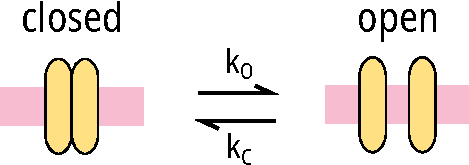
\includegraphics[width=\textwidth]{model_introduction_diagrams.pdf}
	\end{subfigure}
	\hfill
	\begin{subfigure}[t]{0.45\textwidth}
		\caption{}\label{ch4fig:simple_diag_2}
		\centering
		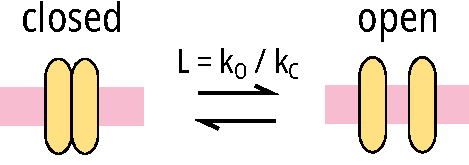
\includegraphics[width=\textwidth]{model_introduction_diagrams_2.pdf}
	\end{subfigure}
	\caption[Simple ion channel model]{
	The transition between two states, open and closed, can be described either by two kinetic constants (\subref{ch4fig:simple_diag_1}) for the opening ($k_O$) and closing ($k_C$), or by an equilibrium constant $L$ (\subref{ch4fig:simple_diag_2}), which is equal to $\frac{k_O}{k_C}$.
	}\label{ch4fig:simple_model_diagram}
\end{figure}

To relate this to empirical measurements of ion channel function, $L$ is equivalent to the $P_O$ of this two-state channel.
Alternatively, in this simple two-state channel, $k_O$ and $k_C$ can be calculated directly by measuring the lifetimes of the closed and open states respectively from single-channel recordings \cite{reinhold_penner_auth_single-channel_1995, sivilotti_praise_2016}.
Of course, real ion channels are more complicated and two states are not sufficient to describe the complexity of the ligand regulation of K\ATP{} channels, which visit a multitude of conformational states.
As our understanding of the channel grows, the more complex a model needs to be to fully account for all observed aspects of function.

One shortcoming of K\ATP{} channel functional models to date is that there are limited data directly measuring binding of nucleotides to the channel, and as such the nucleotide-bound conformational states and transitions of the channel have had to be inferred from electrophysiologcal measurements.
Here, we hope to apply our correlated measurements of nucleotide binding and channel inhibition to reconcile the predictions of existing models of K\ATP{} channel inhibition by nucleotides.

\subsection{Restricting the subset of possible models}

The two classes of models which have been proposed to describe K\ATP{} channel inhibition can be categorised into two groups; models in which each Kir6.2 subunit is able to change between open and closed conformations independently, and models in which opening and closing take place via a concerted mechanism of all four subunits \cite{enkvetchakul_kinetic_2000-1, enkvetchakul_atp_2001, drain_concerted_2004, fang_n-terminal_2006, wang_subunit-stoichiometric_2007, craig_how_2008-1, proks_modeling_2009, vedovato_nucleotide-binding_2015}.
The independent class of models are often referred to as Hodgkin and Huxley (HH)-like models, after the original model proposed to describe voltage-gated ion channels \cite{hodgkin_quantitative_1952}.
The concerted class of models are often referred to as Monod-Wyman-Changeaux (MWC)-like models, after the allosteric model formulated by Monod, Wyman and Changeaux to describe hemoglobin \cite{monod_nature_1965}.

Conceptually, an MWC-like model is easier to reconcile with the structure of K\ATP{} given that each inhibitory nucleotide binding site is composed of domains from two adjacent subunits; it is hard to imagine how nucleotide binding could lead to an indepedent conformational change in one subunit alone \cite{craig_how_2008-1}.
Empirically, the two types of model make testable predictions about channel behaviour and nucleotide binding.
In a concerted model, each nucleotide binding event contributes the same amount of energy towards closure of the pore, such that each subunit binding a nucleotide will have an additive effect on the probability of the channel closing.
In an independent model, as each subunit is free to change its conformation independently, the stochiometry of nucleotide binding is less clear.
Most formulations of an independent model have suggested that K\ATP{} channel behaviour is most consistent with a single nucleotide binding event being sufficient to drive closure of the channel \cite{trapp_molecular_1998, markworth_atp4-_2000, li_open_2002, fang_n-terminal_2006-1}.

A number of studies have examined the kinetics of single K\ATP{} channels to determine which model best describes nucleotide inhibition \cite{drain_concerted_2004, fang_n-terminal_2006-1, wang_subunit-stoichiometric_2007, craig_how_2008-1}.
\cite{drain_concerted_2004} examined single channel currents in patches excised from \textit{Xenopus} oocytes injected with a mixture of Kir6.2\textgreek{D}C and Kir6.2\textgreek{D}C-N160D,T171A subunits.
The T171A mutation appears to eliminate the interburst closures of the Kir6.2\textgreek{D}C by dramatically slowing the rate at which the ATP-sensitive inhibition gate closes.
The authors classified the single channel stoichiometry by assessing the sensitivity of currents to inhibition by spermine, which is provided to a subunit by the N160D mutation.
An exponential relationship between the mean burst time of the channel and the number of mutant subunits incorporated into it fit the predictions made by a concerted model of inhibition.

\citeauthor{wang_subunit-stoichiometric_2007} and \citeauthor{craig_how_2008-1} constructed tetrameric concatemers of Kir6.2 subunits to precisely control the stochiometry of the resulting channels.
The authors introduced mutations which affected either nucleotide binding (K185E \cite{wang_subunit-stoichiometric_2007, craig_how_2008-1}) or mutations which altered intrinsic gating (C166S, T171Y \cite{wang_subunit-stoichiometric_2007}) into a fixed proportion of Kir6.2 subunits in the concatemerised channels.
This selective disruption of individual subunits resulted in changes in ATP-dependent inhibition which could only be explained by a concerted model of K\ATP{} channel inhibition.
However, as these experiments relied on introducing an additional physical linker between Kir6.2 subunits, the observed concerted gating behaviour may in part be due to the concatemerisation.

\section{Implementing an MWC model}

\subsection{A simple case}

The simplest case of an allosteric MWC model for an ion channel is shown as Scheme I in Figure \ref{ch4fig:mwc_model_diagrams}.
This simple case assumes a channel composed of a single monomer with a single binding site for ligand $A$.
The channel is restricted to two functional states, open and closed.
These two states exist in an equilibrium described by L, which is equivalent to $\frac{[open]}{[closed]}$.
Ligand $A$ binds to the protein with a microscopic affinity constant $K_A$.
The ligand $A$ differentially stabilises the open and closed states by a constant $D_A$.
When $D_A$ is unity, the ligand $A$ binds equally to both states and so does not influence the conformational changes of the channel.
When $D_A>1$, the ligand $A$ preferentially stabilises the open state, while when $D_A<1$ the ligand instead preferentially stabilises the closed state.
$D_A$ therefore represents \textit{transduction} of nucleotide binding to channel gating, and vice versa.

For K\ATP{} inhibition, each monomer in Scheme I represents a subunit of Kir6.2, and in our case the ligand $A$ is TNP-ATP.
Expansion of Scheme I to account for four identical subunits is shown in \ref{ch2-methods}.
Importantly, in an MWC model, cooperativity between subunits is not due to the incorporation of an additional paramater, but a phenomenon which arises naturally due to the energetic coupling between ligand binding and channel gating described by the transduction paramater $D_A$.

\begin{figure}[h]
	\centering
	\begin{subfigure}[t]{0.9\textwidth}
		\caption{}\label{ch4fig:mwc_model_diagrams}
		\centering
		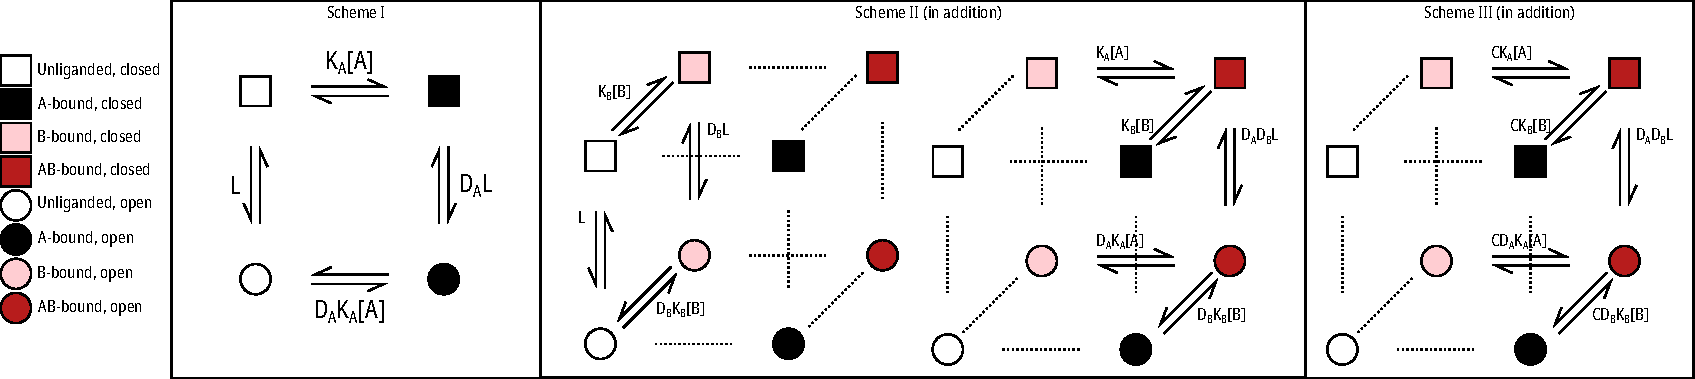
\includegraphics[width=\textwidth]{mwc_model_diagrams.pdf}
	\end{subfigure}
	\vfill
	\begin{subfigure}[t]{0.3\textwidth}
		\caption{}\label{ch4fig:mwc_scheme_1_fits}
		\centering
		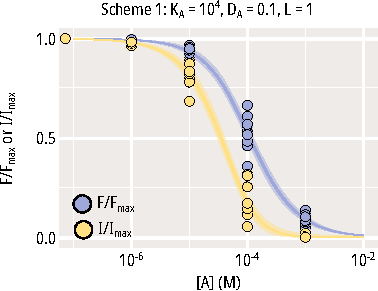
\includegraphics[width=\textwidth]{mwc_scheme_1_fits.pdf}
	\end{subfigure}
	\hfill
	\begin{subfigure}[t]{0.3\textwidth}
		\caption{}\label{ch4fig:mwc_scheme_2_fits}
		\centering
		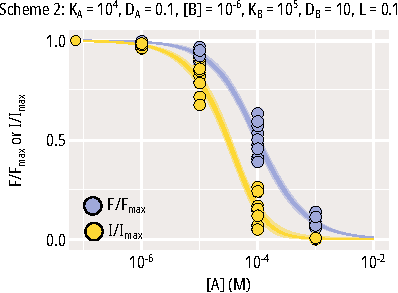
\includegraphics[width=\textwidth]{mwc_scheme_2_fits.pdf}
	\end{subfigure}
	\hfill
	\begin{subfigure}[t]{0.3\textwidth}
		\caption{}\label{ch4fig:mwc_scheme_3_fits}
		\centering
		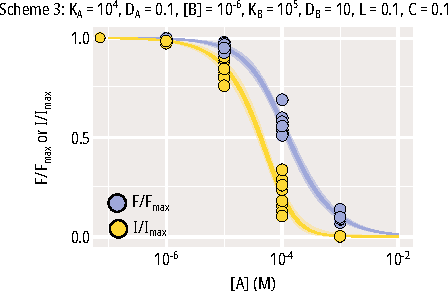
\includegraphics[width=\textwidth]{mwc_scheme_3_fits.pdf}
	\end{subfigure}
	\vfill
	\begin{subfigure}[t]{0.9\textwidth}
		\caption{}\label{ch4fig:mwc_params_1}
		\centering
		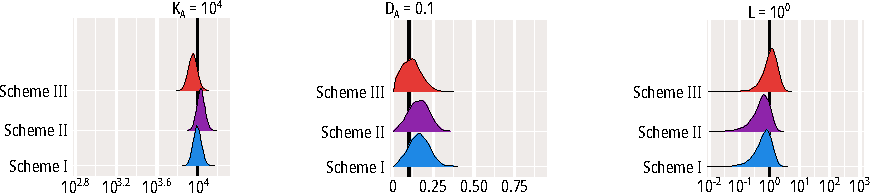
\includegraphics[width=\textwidth]{mwc_scheme_param_fits.pdf}
	\end{subfigure}
	\caption[Generating data from MWC model schemes]{
	\subref{ch4fig:mwc_model_diagrams} Equilibrium diagrams for the three MWC schemes considered.
	For each scheme, only the parameters newly relevant for that scheme are shown explicitly.
	\subref{ch4fig:mwc_scheme_1_fits}, \subref{ch4fig:mwc_scheme_2_fits}, \subref{ch4fig:mwc_scheme_3_fits} Data generated from Scheme I (\subref{ch4fig:mwc_scheme_1_fits}), Scheme II (\subref{ch4fig:mwc_scheme_2_fits}) or Scheme III (\subref{ch4fig:mwc_scheme_3_fits}) all fit to Scheme I.
	The input parameters are shown above each panel.
	$L$ differs between \subref{ch4fig:mwc_scheme_1_fits} and \subref{ch4fig:mwc_scheme_2_fits}, \subref{ch4fig:mwc_scheme_3_fits} due to the introduction of a resting PIP\textsubscript{2} concentration, which in Scheme I is implicitly incorporated into $L$.
	\subref{ch4fig:mwc_params_1} Parameter estimates for the Scheme I model fit to the data generated by all three schemes.
	The input parameter value is marked as a black vertical line for each panel.
	}\label{ch4fig:mwc_models}
\end{figure}

\subsection{The role of PIP\textsubscript{2}}

Of course, nucleotide inhibition is not the only ligand regulation of K\ATP{} channels.
If we assume that activation of K\ATP{} currents by Mg-nucleotides binding at the NBDs of SUR1 or by PIP\textsubscript{2} binding to Kir6.2 are independent processes, the effects of these ligands on nucleotide inhibition can be incorporated implicitly through their effects on $L$.
Mg-nucleotide activation of K\ATP{} channel currents is well described by assuming independence from nucleotide inhibition; i.e. there is no evidence to suggest that there is a direct interaction between binding of Mg-nucleotides to SUR1 and the ability of nucleotides to bind to Kir6.2 \cite{proks_activation_2010-1, vedovato_nucleotide-binding_2015}.
However, there is some evidence to suggest that there is a direct interaction between the nucleotide and PIP\textsubscript{2} binding sites \cite{fan_phosphoinositides_1999, macgregor_nucleotides_2002, proks_modeling_2009, haider_identification_2007}.
The existence of a direct interaction, either by competition for an overlapping binding site or through allosteric rearrangements of the two binding sites, may make it difficult to incorporate regulation by PIP\textsubscript{2} implicitly as an effect on $L$.
We investigated how the existence of direct interaction between the two ligand binding sites may manifest in our observations by simulating data from three progressively expanded MWC-like schemes (Figure \ref{ch4fig:mwc_model_diagrams}).

If we consider introducing a second ligand $B$ which binds to a distinct site on the same monomer and does not directly interact with ligand $A$, we introduce the states shown in Scheme II of Figure \ref{ch4fig:mwc_model_diagrams}.
Each ligand has its own microscopic association constant ($K_A$ or $K_B$) and its transduction factor ($D_A$ or $D_B$).
Importantly, there is no interaction term between ligand $A$ and ligand $B$; the only way the binding of the ligands can impact each other is through effects on $L$.
Scheme II is therefore a restricted form of scheme III, which explicity introduces a term for direct interaction ($C$) between binding sites for ligands $A$ and $B$ on the same monomer.
When $C$ is unity, Scheme III becomes Scheme II.
When $C<1$, binding of one ligand reduces the ability of the other ligand to bind on the same monomer.
When $C>1$, binding of one ligand enhances the ability of the other ligand to bind on the same monomer.

Under Scheme II, in which there is no direct interaction between ligands, changes in the parameters describing ligand $B$ (perturbations of PIP\textsubscript{2} regulation) should manifest in the data in the same way as if there was a change in $L$ in Scheme I \cite{rubin_nature_1966}.
It is unclear whether under Scheme III, with the introduction of the direct interaction $C$, the same assumption is true - and if not, how much it would affect channel behaviour.
To determine whether this approximation is appropriate, we generated data using each of the three schemes in Figure \ref{ch4fig:mwc_model_diagrams} as the underlying model of channel function and then fit the generated observations to Scheme I (Figure \ref{ch4fig:mwc_scheme_1_fits}, \ref{ch4fig:mwc_scheme_2_fits}, \ref{ch4fig:mwc_scheme_3_fits}).
Ten individual sets of observations were generated using the inputs shown above each figure panel as the centre of a lognormal distribution with a standard deviation of 0.25.
These observations were then fit to Scheme I and the values of the three free parameters ($K_A$, $D_A$ and $L$) were estimated (Figure \ref{ch4fig:mwc_params_1}).

\begin{figure}[h]
	\centering
	\begin{subfigure}[t]{0.3\textwidth}
		\caption{}\label{ch4fig:scheme_1_ka_shift}
		\centering
		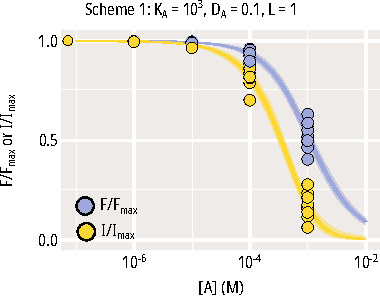
\includegraphics[width=\textwidth]{mwc_scheme_1_ka_shift.pdf}
	\end{subfigure}
	\hfill
	\begin{subfigure}[t]{0.3\textwidth}
		\caption{}\label{ch4fig:scheme_1_da_shift}
		\centering
		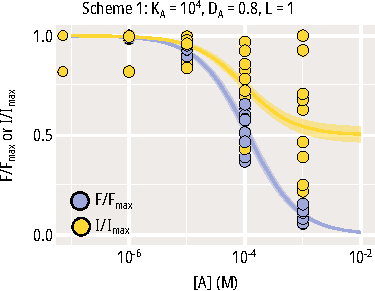
\includegraphics[width=\textwidth]{mwc_scheme_1_da_shift.pdf}
	\end{subfigure}
	\hfill
	\begin{subfigure}[t]{0.3\textwidth}
		\caption{}\label{ch4fig:scheme_1_l_shift}
		\centering
		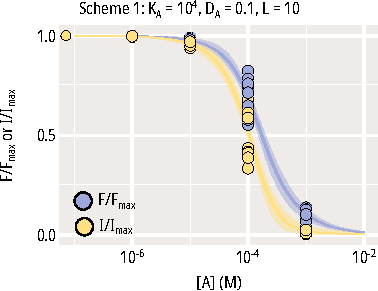
\includegraphics[width=\textwidth]{mwc_scheme_1_l_shift.pdf}
	\end{subfigure}
	\vfill
	\begin{subfigure}[t]{0.9\textwidth}
		\caption{}\label{ch4fig:mwc_params_2}
		\centering
		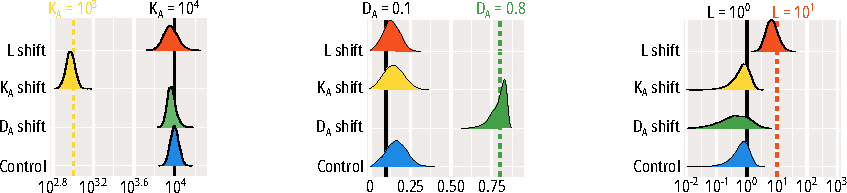
\includegraphics[width=\textwidth]{mwc_scheme_param_fits_2.pdf}
	\end{subfigure}
	\caption[Parameter retrieval from MWC models]{
	\subref{ch4fig:scheme_1_ka_shift}, \subref{ch4fig:scheme_1_da_shift}, \subref{ch4fig:scheme_1_l_shift} Data generated from Scheme I with \subref{ch4fig:scheme_1_ka_shift} $K_A$ shifted from $10^4$ to $10^3$, \subref{ch4fig:scheme_1_da_shift} $D_A$ shifted from $0.1$ to $0.8$, or \subref{ch4fig:scheme_1_l_shift} $L$ shifted from $1$ to $10$.
	\subref{ch4fig:mwc_params_2} Parameter estimates from each of the model fits.
	In each case, the modified parameter is retrieved accurately and no other parameters are affected.
	}\label{ch4fig:scheme_1_shifts}
\end{figure}

We can show that when Scheme II or Scheme III are the underlying data generating model, with ligand $B$ representing PIP\textsubscript{2}, we are still able to extract the true values of $K_A$ and $D_A$ by fitting the generated data to Scheme I (Figure \ref{ch4fig:mwc_models}).
Parameter choices for Scheme II and III are such that the open probability of the channel at 0 [ATP] is still 50\%, equivalent to $L=1$ in Scheme I.

We can also show that when Scheme I is the underlying data generating model, changes in any of the three parameters are easily identified and retrieved by fitting the observed data to Scheme I (Figure \ref{ch4fig:scheme_1_shifts}).
This suggests that introducing mutations or perturbing nucleotide inhibition in any other way which directly affects any of the three parameters of this model would be easily identifiable if Scheme I was the true underlying model.

What if Scheme II or III were the underlying model?
We would still expect changes in the three parameters which exist in Scheme I to be identifiable ($L$, $K_A$ and $D_A$), although $L$ would not represent the true unliganded open/closed equilibrium as we would be estimating an $L$ modified by the resting PIP\textsubscript{2} concentration, $K_B$, $D_B$ and $C$ - in this case, the estimated $L$ parameter in fact represents the ATP-unbound open/closed equilibrium.

\begin{figure}[h]
	\centering
	\begin{subfigure}[t]{0.45\textwidth}
		\caption{}\label{ch4fig:scheme_2_kb_shift}
		\centering
		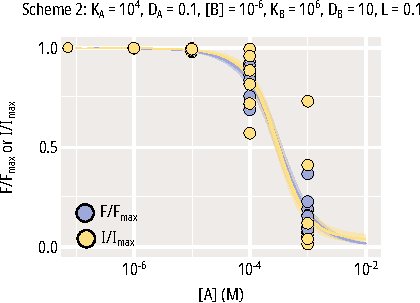
\includegraphics[width=\textwidth]{mwc_scheme_2_kb_shift.pdf}
	\end{subfigure}
	\hfill
	\begin{subfigure}[t]{0.45\textwidth}
		\caption{}\label{ch4fig:scheme_3_kb_shift}
		\centering
		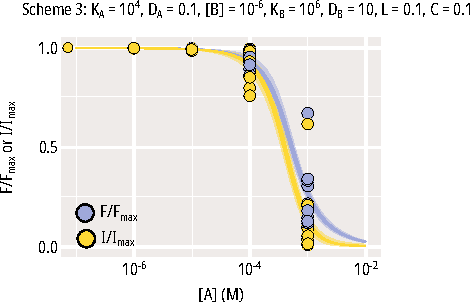
\includegraphics[width=\textwidth]{mwc_scheme_3_kb_shift.pdf}
	\end{subfigure}
	\vfill
	\begin{subfigure}[t]{0.9\textwidth}
		\caption{}\label{ch4fig:mwc_params_3}
		\centering
		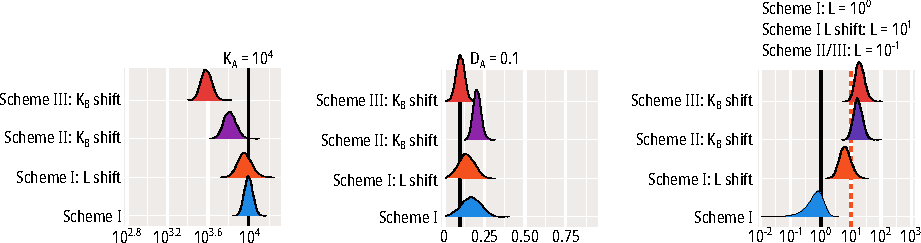
\includegraphics[width=\textwidth]{mwc_scheme_param_fits_3.pdf}
	\end{subfigure}
	\caption[Parameter retrieval from MWC models]{
	\subref{ch4fig:scheme_2_kb_shift}, \subref{ch4fig:scheme_3_kb_shift} Data generated from \subref{ch4fig:scheme_2_kb_shift} Scheme II  or \subref{ch4fig:scheme_3_kb_shift} with $K_B$ shifted from $10^5$ to $10^6$.
	}\label{ch4fig:scheme_2_3_shifts}
\end{figure}

However, it is unclear how changes in parameters which are not explicitly modelled in Scheme I will affect the generated data and the parameter estimates obtained by fitting the data to Scheme I.
Figure \ref{ch4fig:scheme_2_3_shifts} shows the results of increasing $K_B$ by tenfold on data generated from Scheme II (Figure \ref{ch4fig:scheme_2_kb_shift}) or Scheme III (Figure \ref{ch4fig:scheme_3_kb_shift}).
The first observation of note is that the generated data closely resemble those generated from Scheme I when $L$ is increased (Figure \ref{ch4fig:scheme_1_l_shift}), and indeed when the $L$ parameter estimates for a tenfold shift in $K_B$ in Scheme II/III and tenfold shift in $L$ for Scheme I are compared (Figure \ref{ch4fig:mwc_params_3}, right panel) are compared they appear to be similar.
So far so good, as an observed increase in $L$ when fit with Scheme I would lead us to draw the correct inferences about changes in the underlying model (i.e. the open probability of the channel has indeed increased).

However, changes in $K_B$ under Scheme III are not perfectly captured by changes in $L$ when fit to scheme I.
Notably, if a direct interaction exists between the nucleotide and PIP\textsubscript{2} binding site - if Scheme III is the true underlying model - then fitting the observed data to Scheme I would lead us to estimate an incorrect value for $K_A$ (Figure \ref{ch4fig:scheme_2_kb_shift}).
Thus, if there is a direct interaction between the sites, then a mutation which induces an increase in the binding affinity for PIP\textsubscript{2} would not just increase our estimate of $L$ (which would lead to a correct inference) but it would also decrease our estimate of $K_A$ by a not-insignificant amount.
This could lead to the incorrect inference that a mutation is causing a direct change in nucleotide binding when it is in fact causing a direct change in PIP\textsubscript{2} binding, which is influencing our estimates of $K_A$ through a direct interaction with the inhibitory nucleotide binding site.

\subsection{Determining open probability}

As $L$ represents the fraction of channels in the open state, it is directly measurable by determining the channel open probability.
Ideally then, to fit an MWC model to our data we would like to establish the open proability of the channels in our experiments.
Measuring the open probability of an ion channel is most accurately accomplished by single-channel electrophysiological recordings, which allows direct measurement of the time a channel spends in an open state.
Measuring open probability directly is not possible in macroscopic patches, which consist of hundreds or thousands of individual channels.
Thus it would not be possible to determine single channel open probability simultaneously with nucleotide binding, as the fluorescence signal from a small number of channels would be impossible to resolve.

Another approach is noise analysis of currents from large populations of channels \cite{heinemann_7_1992, alvarez_counting_2002}.
The 'noise' in noise analysis refers to current fluctuations which occur when recording from a population of ion channels due to the stochastic channel gating of individual channels.
If there are a constant number of channels ($N$) which are gated independently from each other and share a homogenous open probability ($P_O$) and a single open conductance level ($i$), the observed macroscopic current level $I$ can be described by equation \ref{eq:inpo}:
\begin{equation}\label{eq:inpo}
	I = iNP_O
\end{equation}
and the observed variance of the macroscopic current can be described by the variance of the binomial distribution, equation \ref{eq:bin_1}:
\begin{equation}\label{eq:bin_1}
	\sigma^2 = NP_O \cdot (1 - P_O) \cdot i^2
\end{equation}
where the single channel current is essentially a scaling factor.
If we assume that in a given recording $N$ and $i$ remain constant, and it is $P_O$ which changes in response to any given stimuli, then we can combine equations \ref{eq:inpo} and \ref{eq:bin_1} to yield equation \ref{eq:bin_2}:
\begin{equation}\label{eq:bin_2}
	\sigma^2 = iI - \frac{1}{N} \cdot I^2
\end{equation}
This equation yields a parabola from $I = 0$ to $I = Ni$.
Intuitively, there can be no variance when $P_O$ is exactly 0 or 1, as there will be no opening or closing events which can give rise to current fluctuations.
Once $i$ and $N$ have been determined for a given experiment, the observed current magnitude $I$ can be converted into the $P_O$ for the population of channels by rearranging equation \ref{eq:inpo} as follows:
\begin{equation}\label{eq:poin}
	P_O = \frac{I}{iN}
\end{equation}

Equation \ref{eq:bin_2} can be fit to experimental data by calculating the variance of observed current at different current magnitudes.
This calculation is not exactly trivial, and has been accomplished a number of different ways for different purposes.
For channels with fast inactivation such as the Na\textsubscript{V} family, non-stationary noise analysis involves repeating a stimulus multiple times and measuring variance as the squared sum of deviations from the mean of the current magnitude calculated at the same time point across multiple stimuli, referred to in the literature as an 'isochrone' \cite{sigworth_variance_1980}.
For channels which do not inactivate, stationary noise analysis is possible, and variance can be measured as the squared sum of deviations from the mean current magnitude over a period of time for which $I$ is 'stationary'(Figure \ref{ch4fig:noise_example_1}, \ref{ch4fig:noise_example_2}, \ref{ch4fig:noise_example_3}).

Stationary noise analysis has been performed for K\ATP{} channels before by a number of different researchers \cite{shyng_control_1997, cukras_role_2002, babenko_sur-dependent_2002, tammaro_mutation_2007, pratt_sulfonylurea_2009, proks_activation_2010-1, pratt_engineered_2012-1}.
Unfortunately, in most of the published research the exact procedure for extracting the parameters in equation \ref{eq:bin_1} is described in the methods section, but the quality of the fits and the value of the fitted parameters besides the final calculated $P_O$ is not discussed.
A notable exception to this rule is in reference \cite{tammaro_mutation_2007}, in which two findings are discussed.
Firstly, fitting equation \ref{eq:bin_2} to the mean and variance of \SI{200}{\milli\second} sections of macroscopic currents from wild-type Kir6.2+SUR2A resulted in a systematic underestimation of the single channel current $i$.
From single channel experiments, the single channel current was determined to be \SI{4}{\pico\ampere}, while the value obtained from fitting macroscopic currents was only \SI{2}{\pico\ampere}.
In the case of WT-GFP+SUR1, we see a similar understimation of single channel current (Figure \ref{ch4fig:noise_example_fits_1}, \ref{ch4fig:noise_example_fits_2}, \ref{ch4fig:noise_example_fits_3}), with fits yielding estimates of \SIrange{1.66}{2.64}{\pico\ampere}, while measured single channel currents are at least \SI{4}{\pico\ampere} at a holding potential of \SI{-60}{\milli\volt} \cite{shyng_control_1997, proks_mutations_2001}.
This underestimate of $i$ is most likely due to a reduction in observed channel current variance when compared to the predictions of equation \ref{eq:bin_2}. 

There are two possible explanations for this reduction.
Firstly, the process of filtering and digitising channel currents can lead to underestimates of variance depending on the relationship between the open time of the measured channel and the cut-off frequency of the filter used.
It is unlikely that this phenomenon is responsible for our findings, as the K\ATP{} mean open time duration is close to \SI{1}{\milli\second} and therefore filtering at \SI{5}{\kilo\hertz} would lead to less than a \SI{5}{\percent} underestimation of $i$ \cite{}.
Even if the mean open time of WT-GFP+SUR1 was closer to \SI{0.1}{\milli\second}, we would expect a \SI{20}{\percent} reduction rather than the \SI{50}{\percent} we actually observe.
Empirically, we can use the frequency power spectrum of our measured current fluctuations to determine whether there may be high frequency channel openings we are missing (Figure \ref{ch4fig:spectra_converge}).
For WT-GFP+SUR1, we observe that at frequencies approaching our filter cut-off at \SI{5}{\kilo\hertz} there is very little observed amplitude in active channels when compared to fully inhibited channels, suggesting we are not missing high frequency current fluctuations.

\begin{figure}[h]
	\centering
	\begin{subfigure}[t]{0.3\textwidth}
		\caption{}\label{ch4fig:noise_example_1}
		\centering
		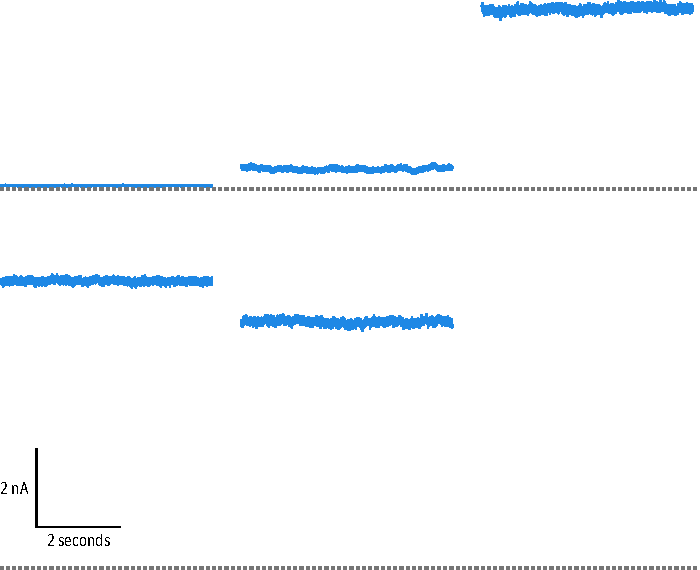
\includegraphics[width=\textwidth]{noise_example_1.pdf}
	\end{subfigure}
	\hfill
	\begin{subfigure}[t]{0.3\textwidth}
		\caption{}\label{ch4fig:noise_example_2}
		\centering
		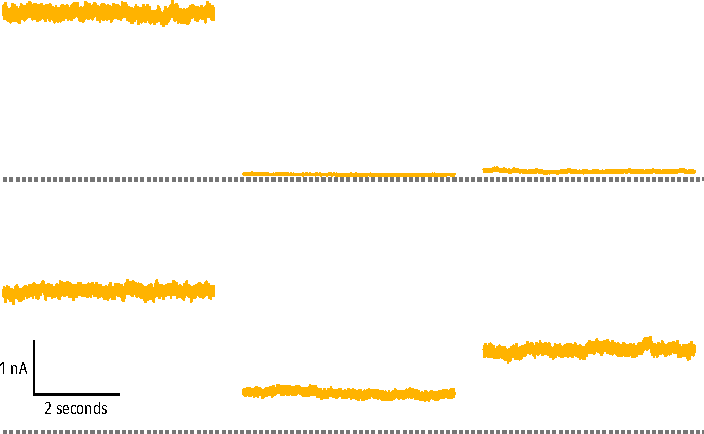
\includegraphics[width=\textwidth]{noise_example_2.pdf}
	\end{subfigure}
	\hfill
	\begin{subfigure}[t]{0.3\textwidth}
		\caption{}\label{ch4fig:noise_example_3}
		\centering
		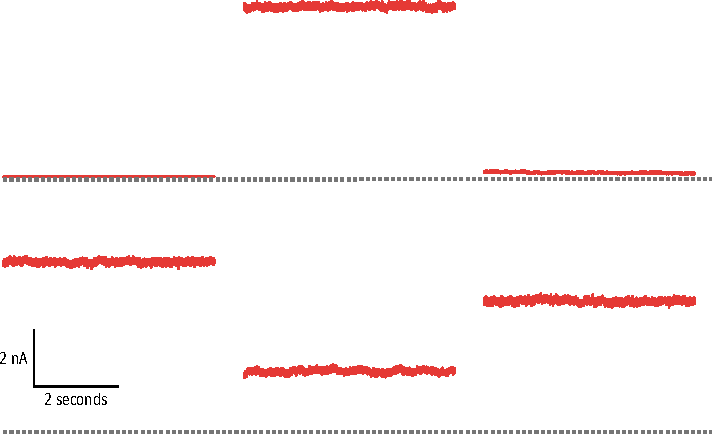
\includegraphics[width=\textwidth]{noise_example_3.pdf}
	\end{subfigure}
	\vfill
	\begin{subfigure}[t]{0.3\textwidth}
		\caption{}\label{ch4fig:noise_example_fits_1}
		\centering
		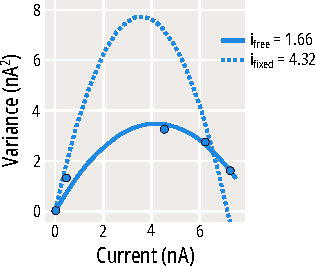
\includegraphics[width=\textwidth]{noise_example_fits_1.pdf}
	\end{subfigure}
	\hfill
	\begin{subfigure}[t]{0.3\textwidth}
		\caption{}\label{ch4fig:noise_example_fits_2}
		\centering
		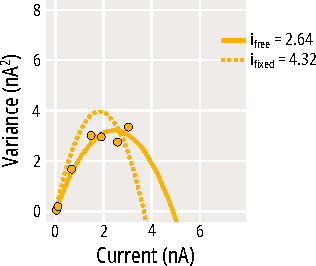
\includegraphics[width=\textwidth]{noise_example_fits_2.pdf}
	\end{subfigure}
	\hfill
	\begin{subfigure}[t]{0.3\textwidth}
		\caption{}\label{ch4fig:noise_example_fits_3}
		\centering
		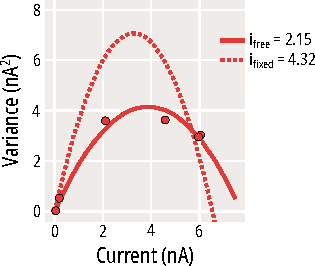
\includegraphics[width=\textwidth]{noise_example_fits_3.pdf}
	\end{subfigure}
	\vfill
	\begin{subfigure}[t]{0.5\textwidth}
		\caption{}\label{ch4fig:spectra_converge}
		\centering
		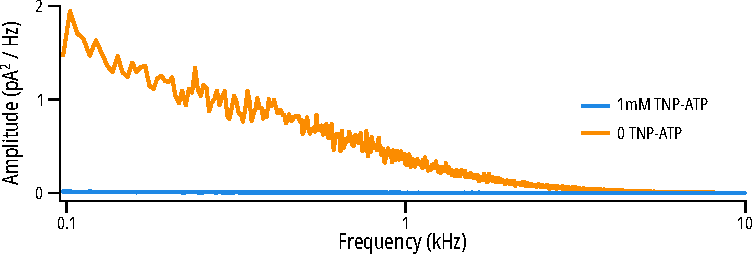
\includegraphics[width=\textwidth]{spectra_converge.pdf}
	\end{subfigure}
	\caption[Systematic underestimation of single channel currents]{
	\subref{ch4fig:noise_example_1},\subref{ch4fig:noise_example_2},\subref{ch4fig:noise_example_3} 5 second extracts from three separate recordings of WT-GFP+SUR1 currents.
	Extracts from different recordings are coloured differently.
	The zero current level determined by barium is indicated as a dashed line.
	\subref{ch4fig:noise_example_fits_1}, \subref{ch4fig:noise_example_fits_2}, \subref{ch4fig:noise_example_fits_3} Plots of the mean current and variance for each of the extracts in the panel above.
	Fits to equation x are shown as a solid line when $i$ is allowed to vary freely, and as a dashed line when $i$ is fixed to \SI{4.32}{\pico\ampere}.
	The fitted value for $i$ is shown for each recording separately.
	\subref{ch4fig:spectra_converge} Averaged power spectra for the three recordings analysed.
	The blue line is the power spectra when channels are fully inhibited and represents the background, while the orange line is the power spectra when channels are most active.
	The high frequency components of the current fluctuations are attenuated to near background levels above \SIrange{2}{3}{\kilo\hertz}.
	}\label{ch4fig:noise_manual}
\end{figure}

Secondly, an underestimation of $i$ could occur due to violations in the underlying assumptions of the binomial distribution.
The first two assumptions are that $N$ and $i$ are constant throughout a recording.
We know that $i$ is unaffected by nucleotide inhibition of K\ATP{} channels, nor is it affected by PIP\textsubscript{2} or channel rundown.
Given that we are recording from excised patches, it is unlikely that there will be any change in the number of channels present in the membrane ($N$) during the short time course of a recording.
The third assumption in using equation \ref{eq:bin_2} is that the channels in a patch share a homogenous $P_O$, which can be perturbed to a similar extent by a stimulus (in our case, application of nucleotide).
This assumption is far harder to justify for our experimental condition, in which channel rundown due to loss of PIP\textsubscript{2} results in a complicated mixture of channel populations with different $P_O$s, which respond differently to nucleotide inhibition.

An extreme case in which channels transition between two states, one where $0 < P_O < 1$ and one where $P_O \approx 0$ can be approximated by equation \ref{eq:bin_1}, with a channel transitioning to the $P_O \approx 0$ state essentially considered to be no longer available to open, reducing $N$.
Thus, fitting the observed current-variance data with \ref{eq:bin_1} would yield a straight line where the slope of the line is equal to $i \cdot (1 - P_O)$.
This formulation of equation \ref{eq:bin_1} has been used successfully in the analysis of currents from CRAC channels \cite{prakriya_regulation_2006}, VSOA channels \cite{jackson_single-channel_1995, jackson_single_1996}, and in the analysis of a specific cardiac K\ATP{} channel mutation \cite{tammaro_mutation_2007}.
Unfortunately, in our case channel rundown does not render the K\ATP{} channel completely unable to open, with fully rundown channels still displaying openings.
Instead of each current measurement being a draw from a single binomial distribution, we are instead drawing from a mixture of binomial distributions with different $P_O$.
We can demonstrate how this could lead to an underestimation of $i$ by simulating a simple case where there are two populations of channels, $a$ and $b$, with a shared single channel conductance $i$ but one with a tenfold lower $P_O$ than the other:

\begin{equation}\label{eq:bibi_sim}
\begin{split}
	N &= 1000 \\
	N &= N_a + N_b \\
	0 < P_{O_{a}} &< 1 \\
	P_{O_{b}} &= \frac{P_{O_{a}}}{10} \\
	i &= 4 \\
	I &= i * Binomial(N_a, P_{O_{a}}) + Binomial(N_b, P_{O_{b}})
\end{split}
\end{equation}

where population $a$ consists of $N_a$ channels with an open probability $P_{O_{a}}$, and population $b$ consists of $N_b$ channels with an open probability $P_{O_{b}}$.

Comparing the mean current/variance relationship of simulated currents from a single binomial (Figure \ref{ch4fig:simulated_noise_1}, \ref{ch4fig:simulated_noise_2}) to that of simulated currents from the mixture of binomials in equation \ref{eq:bibi_sim} (Figure \ref{ch4fig:simulated_noise_3}) reveals that equation \ref{eq:bin_1} is no longer able to retrieve the true values of $i$ and $N$ when the data generating process is not a single binomial distribution.
In fact, the underestimation of $i$ from fitting to data simulated in this way is very similar to the underestimation of $i$ we see when fitting to our measure data (Figure \ref{ch4fig:noise_manual}).

\begin{figure}[h]
	\centering
	\begin{subfigure}[t]{0.3\textwidth}
		\caption{}\label{ch4fig:simulated_noise_1}
		\centering
		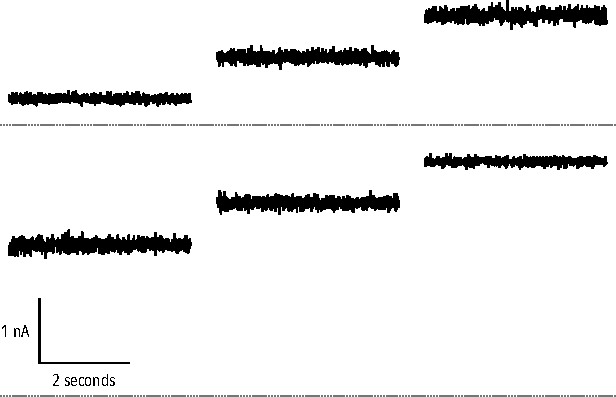
\includegraphics[width=\textwidth]{simulated_noise_1.pdf}
	\end{subfigure}
	\hfill
	\begin{subfigure}[t]{0.3\textwidth}
		\caption{}\label{ch4fig:simulated_noise_2}
		\centering
		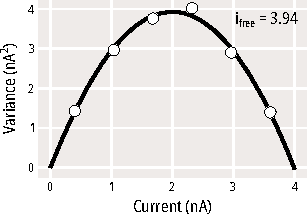
\includegraphics[width=\textwidth]{simulated_noise_2.pdf}
	\end{subfigure}
	\hfill
	\begin{subfigure}[t]{0.3\textwidth}
		\caption{}\label{ch4fig:simulated_noise_3}
		\centering
		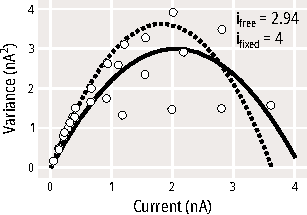
\includegraphics[width=\textwidth]{simulated_noise_3.pdf}
	\end{subfigure}
	\caption[Simulated multibinomial currents]{
	\subref{ch4fig:simulated_noise_1} 5 second segments of simulated channel currents drawn from a single binomial distribution.
	All segments share a common single channel conductance $i$ and number of channels $N$, but the $P_O$ is varied.
	\subref{ch4fig:simulated_noise_2} Fits of equation \ref{eq:bin_2} to the simulated currents in \subref{ch4fig:simulated_noise_1} successfully retrieve an estimate of $i$ which is approximately correct.
	\subref{ch4fig:simulated_noise_3} Fits of equation \ref{eq:bin_2} to segments of currents simulated by drawing from a mixture of two binomial distributions with different baseline $P_O$s.
	The estimate for $i$ retrieved by letting the parameter vary is much lower than the actual value for $i$.
	Fixing $i$ to the correct value results in a fit which underestimates the number of channels $N$.
	}\label{ch4fig:noise_sim}
\end{figure}

We considered whether the underestimation of $i$ and the poor fits to equation \ref{eq:bin_2} when $i$ was fixed to \SI{4.32}{\pico\ampere} (Figure \ref{ch4fig:noise_manual}) may be due to the low number of data points when selecting segments of current manually.
We took our full current records from each excised patch from cells expressing WT-GFP+SUR1 or W311*-GFP+SUR1, divided them into 1 second segments, and plotted the mean current/variance relationship for each segment (Figure \ref{ch4fig:noise_fits_1}).
We fit the data to equation \ref{eq:bin_2} either with $i$ allowed to vary freely, or with $i$ fixed to \SI{4.32}{\pico\ampere}.
Our estimates for $i$ when it was allowed to vary freely were similar to our estimates from Figure \ref{ch4fig:noise_manual}, with no patch yielding a value above \SI{3}{\pico\ampere} (Figure \ref{ch4fig:noise_fits_2}).
The fits with $i$ fixed to \SI{4.32}{\pico\ampere} clearly fit the data less well, and the resulting estimate for the open probability on patch excision exceeded 1 for nearly every patch, which is of course not possible.

\begin{figure}[h]
	\centering
	\begin{subfigure}[t]{0.9\textwidth}
		\caption{}\label{ch4fig:noise_fits_1}
		\centering
		\includegraphics[width=\textwidth]{noise_fits_1.pdf}
	\end{subfigure}
	\vfill
	\begin{subfigure}[t]{0.9\textwidth}
		\caption{}\label{ch4fig:noise_fits_2}
		\centering
		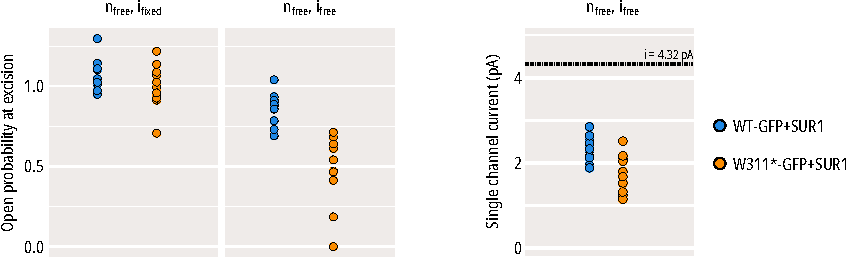
\includegraphics[width=\textwidth]{noise_fits_2.pdf}
	\end{subfigure}
	\caption[Estimating open probability from stationary noise analysis]{
	\subref{ch4fig:noise_fits_1} Plots of the mean current and variance for 1 second extracts from recordings of WT-GFP+SUR1 (blue) or W311*-GFP+SUR1 (orange).
	Fits to equation x are shown as a solid line when $i$ is allowed to vary freely, and as a dashed line when $i$ is fixed to \SI{4.32}{\pico\ampere}.
	\subref{ch4fig:noise_fits_2} Parameter estimates from fits in \subref{ch4fig:noise_fits_1} are shown as separate points for each experiment.
	For fits to equation \ref{eq:bin_2}, open probability is calculated from the intial current on patch excision.
	}\label{ch4fig:all_noise_fits}
\end{figure}

Given these results, we chose not to use noise analysis to calculate the $P_O$ directly for each patch.
In addition, \citeauthor{cukras_role_2002} compared the $P_O$ calculated from noise analysis and the $P_O$ calculated by application of saturating concentrations of PIP\textsubscript{2} of a variety of K\ATP{} channel mutants, and found only a weak correlation between the two methods \cite{cukras_role_2002}.

\subsection{Comparing models}

We expanded Scheme I from Figure \ref{ch4fig:mwc_model_diagrams} to account for the four inhibitory nucleotide binding sites of K\ATP{} (Figure \ref{ch4fig:model_expansion_1}).
In addition, we considered an alternate model in which only the first nucleotide binding event contributes towards closure of the channel, and thus there is no cooperativity between subunits (Figure \ref{ch4fig:model_expansion_2}).
We then fit our observed TNP-ATP binding and current inhibition data from excised patches expressing W311*-GFP+SUR1 to equations \ref{eq:mwc_binding} and \ref{eq:normalised_po} respectively.

\begin{figure}[h]
	\centering
	\begin{subfigure}[t]{0.9\textwidth}
		\caption{}\label{ch4fig:model_expansion_1}
		\centering
		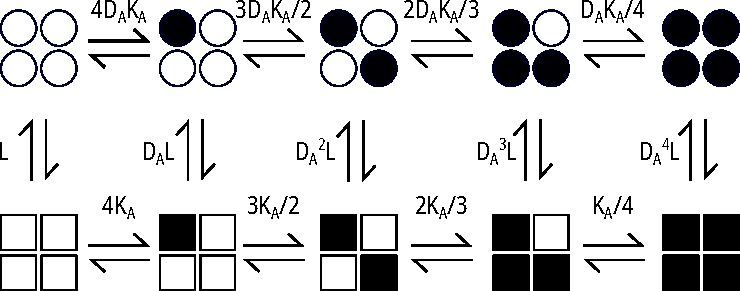
\includegraphics[width=\textwidth]{mwc_scheme_1_expansion.pdf}
	\end{subfigure}
	\vfill
	\begin{subfigure}[t]{0.9\textwidth}
		\caption{}\label{ch4fig:model_expansion_2}
		\centering
		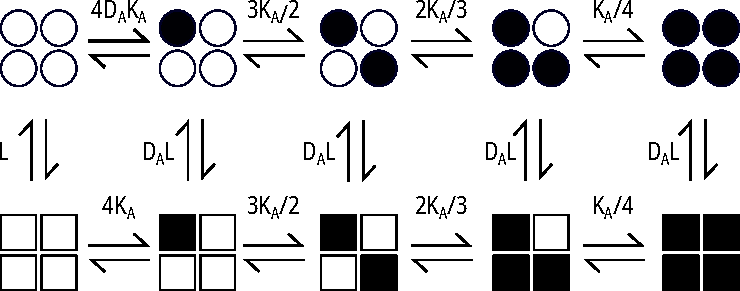
\includegraphics[width=\textwidth]{mwc_scheme_1_expansion_2.pdf}
	\end{subfigure}
	\caption[Full model diagrams]{
	Equilibrium diagrams for the two models considered.
	\subref{ch4fig:model_expansion_1} is the concerted MWC model in which each nucleotide binding event contributes towards closing (described by the $D_A$ term modifying each binding event).
	\subref{ch4fig:model_expansion_1} is an alternate single binding model in which only the first nucleotide binding event contributes towards closing.
	}\label{ch4fig:model_compare}
\end{figure}

Both models fit our data reasonably well (Figure \ref{ch4fig:w311_model_comparison}), although the posterior distributions of the fits to the MWC model (Figure \ref{ch4fig:w311_mwc_fit_1}, \ref{ch4fig:w311_mwc_fit_2}) are narrower than those for the single binding model (Figure \ref{ch4fig:w311_single_fit_1}, \ref{ch4fig:w311_single_fit_2}).
Examining the posterior distributions for the three parameters, both models yield similar estimates, with much narrow distributions for $K_A$ than for $D_A$ and $L$ (Figure \ref{ch4fig:w311_mwc_fit_3}).
We compared the ability of the two models to explain the data with two complimentary methods.
First, we used bridge sampling to calculate a Bayes factor of \num{1.1e4} in favor of the MWC model over the single binding model \cite{gronau_bridgesampling_2020}.
The Bayes factor can be interpreted as the weight of evidence in favour of one model over another \cite{wagenmakers_practical_2007}.
Specifically, the observed data are \num{1.1e4} more likely to have occured under the MWC model than they are under the single binding model.
In addition, we performed leave-one-out cross-validation (LOO-CV), which approximates the out-of-sample predictive accuracy of each of the fitted models \cite{vehtari_practical_2017}.
The MWC model fit has a higher expected predictive accuracy than the single binding model (elpd difference of \num{27.3 (63)}).
Together, the Bayes factor and LOO-CV scores favour a concerted MWC binding model.

The \SI{95}{\percent} intervals for the $K_A$ are \SIrange{9e3}{1.7e4}{\per\Molar} for the MWC model, corresponding to a $K_d$ of \SIrange{56}{110}{\micro\Molar}.

\begin{figure}[h]
	\centering
	\begin{subfigure}[t]{0.45\textwidth}
		\caption{}\label{ch4fig:w311_mwc_fit_1}
		\centering
		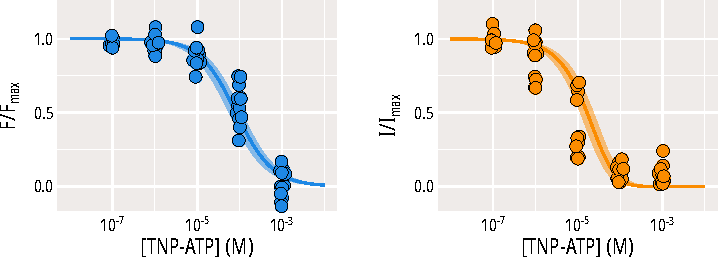
\includegraphics[width=\textwidth]{w311_mwc_fit_1.pdf}
	\end{subfigure}
	\hfill
	\begin{subfigure}[t]{0.45\textwidth}
		\caption{}\label{ch4fig:w311_mwc_fit_2}
		\centering
		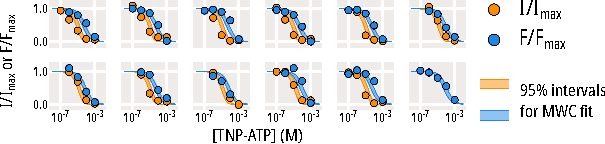
\includegraphics[width=\textwidth]{w311_mwc_fit_2.pdf}
	\end{subfigure}
	\vfill
	\begin{subfigure}[t]{0.45\textwidth}
		\caption{}\label{ch4fig:w311_single_fit_1}
		\centering
		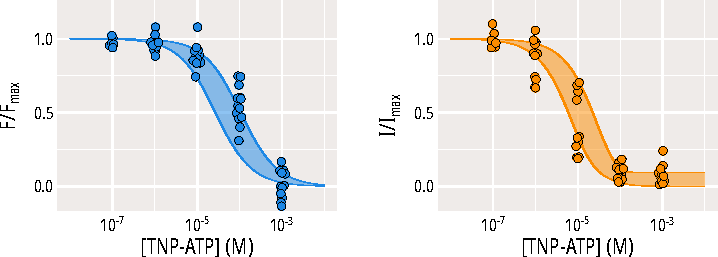
\includegraphics[width=\textwidth]{w311_single_fit_1.pdf}
	\end{subfigure}
	\hfill
	\begin{subfigure}[t]{0.45\textwidth}
		\caption{}\label{ch4fig:w311_single_fit_2}
		\centering
		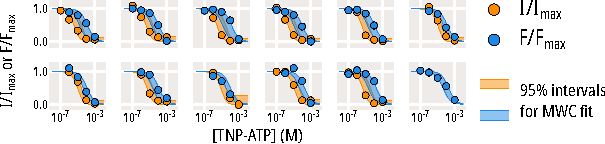
\includegraphics[width=\textwidth]{w311_single_fit_2.pdf}
	\end{subfigure}
	\vfill
	\begin{subfigure}[t]{0.9\textwidth}
		\caption{}\label{ch4fig:w311_mwc_fit_3}
		\centering
		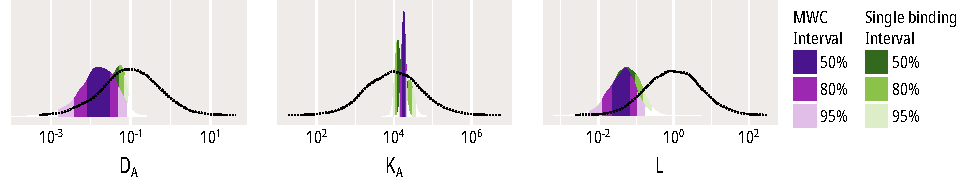
\includegraphics[width=\textwidth]{w311_mwc_fit_3.pdf}
	\end{subfigure}
	\caption[A concerted model explains the data better than an independent model]{
	\subref{ch4fig:w311_mwc_fit_1} Current inhibition (orange) and fluorescence quenching (blue) by TNP-ATP of W311*-GFP+SUR1 in excised patches, data the same as Figure \ref{ch3fig:pcf_1}.
	Fitted curves are the \SI{95}{\percent} intervals of the posterior probability distribution of fits to the MWC model paramaterised in equations \ref{eq:mwc_binding} and \ref{eq:normalised_po}, not including the $\delta_{experiment}$
	\subref{ch4fig:w311_mwc_fit_2} Each experiment from \subref{ch4fig:w311_mwc_fit_1} is plotted separately.
	The fitted curves represent the \SI{95}{\percent} intervals of the posterior probability distribution including the $\delta_{experiment}$.
	\subref{ch4fig:w311_single_fit_1} Current inhibition (orange) and fluorescence quenching (blue) by TNP-ATP of W311*-GFP+SUR1 in excised patches, data the same as Figure \ref{ch3fig:pcf_1}.
	Fitted curves are the \SI{95}{\percent} intervals of the posterior probability distribution of fits to the single binding model paramaterised in equation x, not including the $\delta_{experiment}$
	\subref{ch4fig:w311_single_fit_2} Each experiment from \subref{ch4fig:w311_single_fit_1} is plotted separately.
	The fitted curves represent the \SI{95}{\percent} intervals of the posterior probability distribution including the $\delta_{experiment}$.
	\subref{ch4fig:w311_mwc_fit_3} Posterior probability distributions for each of the three free parameters estimated from fits to the MWC model (blue) or the single binding model (orange) are shown shaded according to their intervals.
	The prior distributions for each of the parameters are shown as a dashed line.
	}\label{ch4fig:w311_model_comparison}
\end{figure}